\documentclass[11pt]{article}
\usepackage[margin=2cm]{geometry}
\usepackage{amssymb,amsmath}
\usepackage{graphicx}
\usepackage{multicol}
\usepackage{algorithm,algpseudocode}

\title{Multigrid Monte Carlo sampling from posterior distributions}
\author{Eike Mueller, University of Bath}

\begin{document}
\maketitle
%%%%%%%%%%%%%%%%%%%%%%%%%%%%%%%%%%%%%%%%%%%%%%%%%%%%%%%%%%%%%%%%%%%%%%%%%%%%%%
\section{Problem setup}
%%%%%%%%%%%%%%%%%%%%%%%%%%%%%%%%%%%%%%%%%%%%%%%%%%%%%%%%%%%%%%%%%%%%%%%%%%%%%%
The prior is a multivariate normal distribution $\mathcal{N}(0,Q^{-1})$ with mean $\overline{x}=0$ and precision matrix $Q$ that is obtained by discretising the following positive definite linear operator $\mathcal{L}$ with the finite-volume method on a lattice with $m\times m$ cells:
\begin{equation}
    \mathcal{L} u = -\nabla (K(z_1,z_2) \nabla u) + b(z_1,z_2) u \qquad\text{for $z = (z_1,z_2) \in [0,1]\times [0,1]$}.
\end{equation}
For simplicity, periodic boundary conditions are applied. The number of unknowns is $n=m^2$ and $Q$ is an $n\times n$ matrix. The scalar fields $K(z_1,z_2)$ and $b(z_1,z_2)$ are given by
\begin{equation}
    \begin{aligned}
        K(z_1,z_2) & =\alpha _K + \beta_K \sin(2 \pi  z_1) \sin(2 \pi  z_2) \\
        b(z_1,z_2) & =\alpha _b + \beta_b \cos(2 \pi  z_1) \cos(2 \pi  z_2)
    \end{aligned}
\end{equation}
where
\begin{xalignat}{4}
    \alpha_K &= 1.5, &
    \beta_K &= 0.3, &
    \alpha_b &= 1.2, &
    \beta_b &= 0.1.
\end{xalignat}
The field $u$ is measured at $N=8$ locations, i.e. we assume that we can have measured the field $u$ to be $y_1,y_2,\dots,y_N$ at these locations and the covariance of the measurements is given by the (not necessarily diagonal) $N\times N$ matrix $\Sigma$. Write $X\in\mathbb{R}^n$ for the prior RV, which encodes the values of the field $u(z_1,z_2)$ in the grid cells. We have that
\begin{equation}
    Y = B^TX + E
\end{equation}
where $E\sim \mathcal{N}(0,\Sigma)$ and the tall, skinny $n\times N$ matrix $B$ encodes the measurement operator. We want to sample from the posterior distribution $\pi(X|y)$. The quantity $Q$ of interest that we consider here is the measurement of $X$ at a fixed sample location. Fig. \ref{fig:mean_variance} shows the sample mean and sample variance of the posterior distribution.
\begin{figure}
    \begin{center}
        \begin{minipage}{0.45\linewidth}
            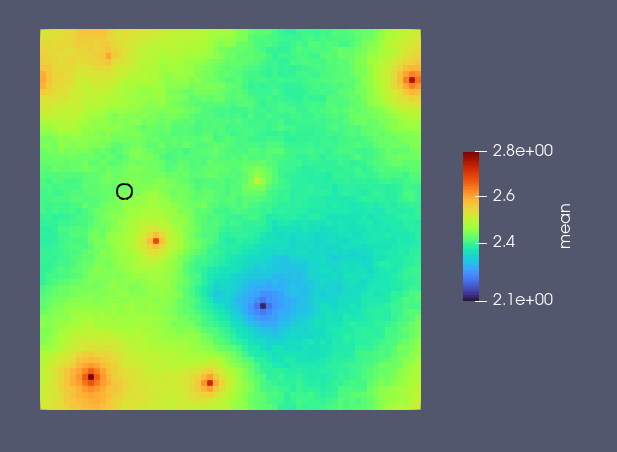
\includegraphics[width=\linewidth]{mean.png}
        \end{minipage}
        \hfill
        \begin{minipage}{0.45\linewidth}
            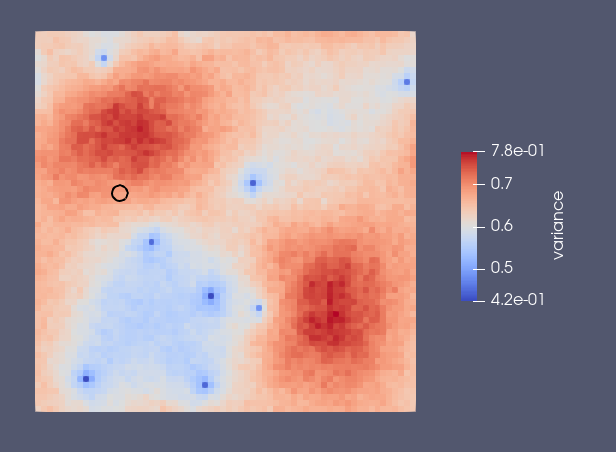
\includegraphics[width=\linewidth]{variance.png}
        \end{minipage}
    \end{center}
    \caption{Sample mean (left) and sample variance (right) of the posterior distribution for a $64\times 64$ lattice. The location where the quantity of interest is measured is marked by a circle. The data was generated with the Multigrid Monte Carlo sampler}
    \label{fig:mean_variance}
\end{figure}
%%%%%%%%%%%%%%%%%%%%%%%%%%%%%%%%%%%%%%%%%%%%%%%%%%%%%%%%%%%%%%%%%%%%%%%%%%%%%%
\section{Samplers}
%%%%%%%%%%%%%%%%%%%%%%%%%%%%%%%%%%%%%%%%%%%%%%%%%%%%%%%%%%%%%%%%%%%%%%%%%%%%%%
We consider three samplers to draw from the posterior distribution $\mathcal{N}(x_{\text{post}},A^{-1})$ where $A = Q + B\Sigma^{-1}B^T$ and $x_{\text{post}} = \overline{x} + Q^{-1}B(\Sigma + B^T Q^{-1}B)^{-1}(y-B^T\overline{x})=:A^{-1}f$ (recall that the prior mean is $\overline{x}=0$):
\begin{description}
    \item[Cholesky.] Compute the sparse Cholesky factorisation $LL^T$ of the precision matrix $Q+B\Sigma^{-1}B$. Of course, this is only done once before the sampling process and we do not include it in the timings reported below. Draw samples $\xi\in\mathbb{R}^n$ from a multivariate normal distribution with zero and unit covariance matrix. Solve the triangular systems $Lg = f$ and then $L^T x = (\xi + g)$ to obtain an independent sample $x$.
    \item[SSOR.] Use a symmetric overrelaxation sampler with overrelaxation factor $\omega=1$ to generate a new sample $x^{k+1}$ from the current state $x^x$ in the Markov chain. Note that since $\omega=1$ this is just a forward Gauss-Seidel sweep followed by a backward Gauss-Seidel sweep.
    \item[MultigridMC.] The next sample is obtained from the current sample with the Multigrid Monte Carlo algorithm. Construct a multigrid hierarchy and coarsen the operator with bilinear interpolation. The pre-sampler on each level is forward SOR and the post-sampler is backward SOR; $\omega=1$ is the overrelaxation factor for both smoothers so again this reduces to Gauss-Seidel in this special case. The number of levels is chosen such that the coarsest grid has the size $2\times 2$ and a Cholesky sampler is used on this level. Note that the work on the finest level (one forward SOR sweep followed by on backward SOR sweep) is identical to the total work in the SSOR sampler.
\end{description}
%%%%%%%%%%%%%%%%%%%%%%%%%%%%%%%%%%%%%%%%%%%%%%%%%%%%%%%%%%%%%%%%%%%%%%%%%%%%%%
\section{Numerical results}
%%%%%%%%%%%%%%%%%%%%%%%%%%%%%%%%%%%%%%%%%%%%%%%%%%%%%%%%%%%%%%%%%%%%%%%%%%%%%%
The samplers were run for grids of size $32\times 32$, $64\times 64$, $128\times 128$ and $256\times 256$. In each case, after discarding $n_{\text{warmup}}$ samples, a timeseries of the field value at the measurement location (marked by a circle in Fig. \ref{fig:mean_variance}) is recorded over $n_{\text{samples}}=10000$ steps in the Markov chain.
%%%%%%%%%%%%%%%%%%%%%%%%%%%%%%%%%%%%%%%%%%%%%%%%%%%%%%%%%%%%%%%%%%%%%%%%%%%%%%
\subsection{Timeseries and autocorrelation}
%%%%%%%%%%%%%%%%%%%%%%%%%%%%%%%%%%%%%%%%%%%%%%%%%%%%%%%%%%%%%%%%%%%%%%%%%%%%%%
Fig. \ref{fig:timeseries} shows the first steps of this timeseries for different lattice sizes and the three considered samplers.
\begin{figure}
    \begin{center}
        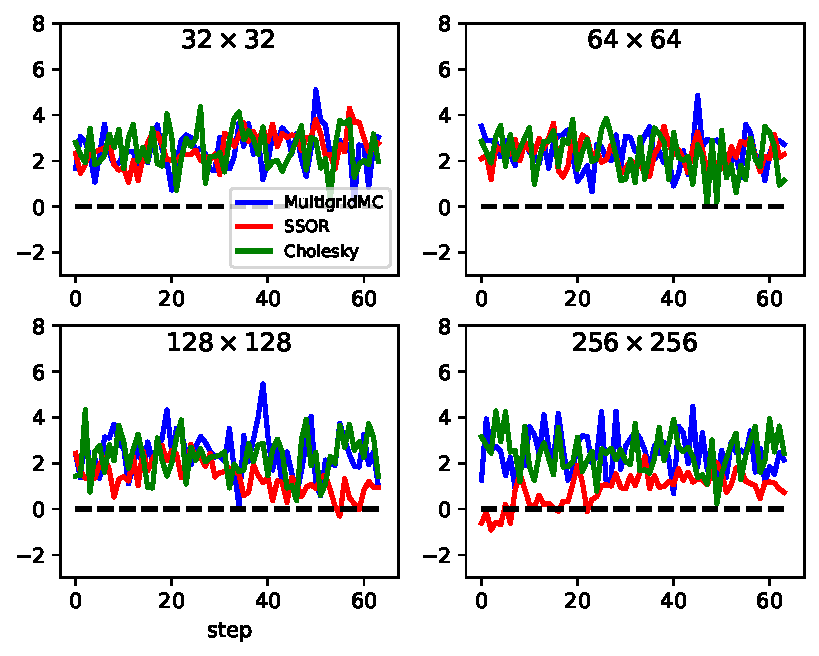
\includegraphics[width=0.7\linewidth]{timeseries.pdf}
        \caption{Sequence of first 64 samples (after warmup) in the Markov chain for different samplers and lattice sizes.}
        \label{fig:timeseries}
    \end{center}
\end{figure}
Writing $x^j$ for the $j$-the state in the Markov chain, the autocorrelation function for lag $k$ is defined as
\begin{equation}
    C(k) = \frac{1}{n_{\text{samples}}-k}\sum_{j=1}^{n_\text{samples}-k} x^{j} x^{j+k}
\end{equation}
The normalised autocorrelation functions $C(k)/C(0)$ are shown for the different samplers in Fig. \ref{fig:autocorrelation}.
\begin{figure}
    \begin{center}
        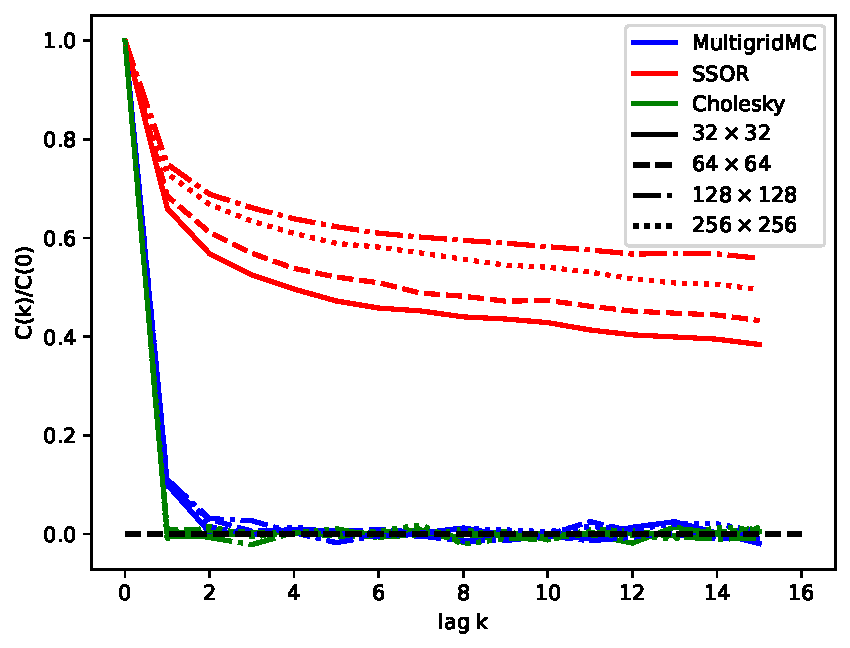
\includegraphics[width=0.7\linewidth]{autocorrelation.pdf}
        \caption{Normalised autocorrelation function for different samplers and lattice sizes.}
        \label{fig:autocorrelation}
    \end{center}
\end{figure}
As this figure shows, the Cholesky sampler generates independent samples. The samples obtained with the SSOR method are strongly correlated, in particular for larger lattice sizes (the autocorrelation function for the $256\times 256$ lattice appears to decay slower than for the $128\times 128$ lattice, but this could be due to the fact that it is estimated with a finite number of samples). For the MultigridMC sampler we show the integrated autocorrelation time (IACT) $\tau_{\text{int}}$ in Tab. \ref{tab:tau_int}
\begin{table}
    \begin{center}
        \begin{tabular}{cc}
            \hline
            lattice         & $\tau_{\text{int}}$ \\
            \hline\hline
            $32 \times 32$  & $1.21 \pm  0.02$    \\
            $64\times 64$   & $1.26 \pm 0.02$     \\
            $128\times 128$ & $1.28 \pm  0.02$    \\
            $256\times256$  & $1.23 \pm  0.02$    \\
            \hline
        \end{tabular}
        \caption{Integrated autocorrelation time for the Multigrid Monte Carlo sampler on different lattices.}
        \label{tab:tau_int}
    \end{center}
\end{table}
Crucially, the IACT does not increase with resolution. Based on the measured values, we expect that the Multigrid MC sampler will generate approximately independent samples if the Markov chain is subsampled with a factor of about $2-3$.
%%%%%%%%%%%%%%%%%%%%%%%%%%%%%%%%%%%%%%%%%%%%%%%%%%%%%%%%%%%%%%%%%%%%%%%%%%%%%%
\subsection{Runtimes}
%%%%%%%%%%%%%%%%%%%%%%%%%%%%%%%%%%%%%%%%%%%%%%%%%%%%%%%%%%%%%%%%%%%%%%%%%%%%%%
\begin{table}
    \begin{center}
        \begin{tabular}{crrr}
            \hline
            lattice         & \multicolumn{1}{c}{Cholesky} & \multicolumn{1}{c}{SSOR} & \multicolumn{1}{c}{Multigrid MC} \\
            \hline\hline
            $32\times 32$   & $0.1438$                     & $0.1038$                 & $0.1712$                         \\
            $64\times 64$   & $1.6852$                     & $0.4070$                 & $0.6608$                         \\
            $128\times 128$ & $16.2871$                    & $1.6529$                 & $2.7176$                         \\
            $256\times 256$ & $120.3880$                   & $8.7008$                 & $13.6875$                        \\
            \hline
        \end{tabular}
        \caption{Measured time per sample for different samplers and lattice sizes. All times are given in milliseconds.}
        \label{tab:runtimes}
    \end{center}
\end{table}
Note that in two dimensions we expect the time for the Cholesky sampler to grow like $\mathcal{O}(N^{3/2})$, whereas the growth is $\mathcal{O}(N)$ for the SSOR and Multigrid MC samplers. When the resolution is double in both dimensions, the runtime for the latter two samplers should increase by a factor four, whereas it should grow by a factor eight for the Cholesky sampler. More generally, in $d$ spatial dimensions the Cholesky solver should cost $\mathcal{O}(N^{2-1/d})$ per sample, whereas the cost is $\mathcal{O}(N)$ independent of $d$ for SSOR and Multigrid MC.
\end{document}
